\documentclass[]{report}

\usepackage{caption}
\usepackage{color}
\usepackage{ctex}
\usepackage{enumerate}
\usepackage{fontspec}
\usepackage[bottom]{footmisc}
\usepackage{graphicx}
\usepackage[breaklinks,colorlinks,linkcolor=black,citecolor=black,urlcolor=black]{hyperref}
\usepackage{listings}
%\usepackage{titlesec}

%修改命名
\renewcommand{\chaptername}{}
\renewcommand{\partname}{}
%\titleformat{\chapter}[block]{\Large\bf}{\chaptername}{20pt}{}

%代码高亮设置
\lstset{
    basicstyle=\small\ttfamily\fontspec{DejaVu Sans Mono},
    %numbers=left,
    %numbersep=5pt,
    %xleftmargin=20pt,
    frame=tb,
    %framexleftmargin=20pt,
    %numberstyle=\footnotesize\color[rgb]{0.5,0.5,0.5},
    keywordstyle=\color[RGB]{40,40,255},
    commentstyle=\it\color[RGB]{0,96,96},
    stringstyle=\rmfamily\slshape\color[RGB]{128,0,0}
}
\renewcommand*\thelstnumber{\arabic{lstnumber}:}
\DeclareCaptionFormat{mylstcap}{\hrule height1.5pt#1#2#3}
\captionsetup[lstlisting]{format=mylstcap,labelfont=bf,singlelinecheck=off,labelsep=space}
\renewcommand{\lstlistingname}{代码}% Listing -> Algorithm
\renewcommand{\lstlistlistingname}{\lstlistingname列表}% List of Listings -> List of Algorithms
%\floatname{algorithm}{算法}


% Title Page
\title{操作系统课程设计报告}
\author{陈宇翔201605301353}


\begin{document}
\maketitle

\tableofcontents

\part{要求回顾}

\chapter{实验内容与任务}

\section{任务}

\subsubsection*{该实验以Linux0.11为例帮助学生探索操作系统的结构、方法和运行过程,理解计算机软件和硬件协同工作的机制。学生需要完成4项任务:}
\begin{enumerate}[(1)]
    \item 分析Linux0.11系统源代码,了解操作系统的结构和方法。
    \item 通过调试、输出运行过程中关键状态数据等方式,观察、探究Linux系统的运行过程。
    \item 建立合适的数据结构,描述Linux0.11系统运行过程中的关键状态和操作,记录系统中的这些关键运行数据,形成系统运行日志。
    \item 用图形表示计算机系统中的各种软、硬件对象,如内存、CPU、驱动程序、键盘、中断事件等等。根据已经产生的系统运行日志,以动画的动态演示系统的运行过程。
\end{enumerate}

\section{工作内容}

\subsubsection*{将整个系统的运行过程可视化需要付出巨大的工作量,一个学期内难以完成。在全面分析源代码的基础上,学生可以根据自身的能力和兴趣在不同层次、规模、难度上完成本项实验:}
\begin{enumerate}[(1)]
    \item 学生可以探究系统某个模块的某个过程,如文件系统的读操作、键盘的输入、CPU的调度等。
    \item 学生可以选择组成大小不等的团队参与实验。
    \item 在可视化处理上,学生也可以做适当的简化。
\end{enumerate}

\chapter{实验过程及要求}

\section{实验前一学期}

在操作系统原理课程中,教师介绍Linux0.11源码结构及相关资料,并公布下一学期操作系统课程设计的任务。学生具备了自己分析源代码的基础。

\section{实验学期}

\subsection{第1-4周,16课时}
将Linux0.11源代码分成基础模块和选读模块,学生必须分析基础模块,然后从选读模块中选择感性趣的模块重点分析。
\subsection{第5-6周,8课时}
学生自由组合成团队,提出设计方案,每个团队说明感兴趣的系统运行过程。
\subsection{第7周,4课时}
讨论、评估设计方案。
\subsection{第8-11周,16课时}
从感兴趣的系统运行过程中提取系统运行的状态数据,并生成系统运行日志。
\subsection{第12-14周,12课时}
根据日志实现运行过程的可视化。
\subsection{15-16周,8课时}
学生演示运行结果,评定成绩。

\chapter{相关知识及背景}

\section{实验以Linux操作系统为背景,涉及}
\begin{enumerate}[-]
    \item 操作系统原理(80\%)
    \item 计算机组成(30\%)
    \item 计算机体系结构(30\%)
    \item C语言(80\%)
    \item 数据结构(30\%)等课程中的基本知识和方法
\end{enumerate}

\section{通过实验学生的如下方面的能力将得到训练和发展}
\begin{enumerate}[(1)]
    \item 代码分析能力
    \item 编程能力
    \item 计算机系统能力
    \item 沟通协作能力
    \item 表达能力
\end{enumerate}

\chapter{教学目的}
\begin{enumerate}[(1)]
    \item 将操作系统原理与具体实现相结合,加深对理论知识的理解
    \item 掌握计算机系统的硬软件整体架构,培养学生的全局观和系统能力
    \item 理解运行中的系统,锻炼学生解决实际问题的能力
\end{enumerate}

\chapter{实验原理及方案}

该实验是一个综合性很强的课程设计,包含了计算机系统中硬件和软件设计的多项基本原理:
\begin{enumerate}[-]
    \item CPU结构
    \item CPU管理
    \item 内存管理
    \item 外设控制
    \item 文件系统
\end{enumerate}

\section{实验的总体思路}
\begin{enumerate}[(1)]
    \item 在代码级别上理解系统的运行过程;
    \item 获取系统运行过程的数据;
    \item 演示系统运行的过程。该实验的结果是开放的,解决具体问题的思路依赖于学生各自的设计目标。
\end{enumerate}

\section{实验可能采用的关键技术}

内核编程技术,用以从内核中输出运行时数据,需要修改内核。其难点在于新增加的代码应该保持内核运行时原有的样子,而且内核编程与普通编程相比,受到更多的限制。

可视化技术,即如何利用图形图像表达系统的运行过程。

\chapter{实验报告要求}
\begin{enumerate}[(1)]
    \item Linux0.11系统源代码分析报告,说明学生本人分析代码的体会及重点分析的代码描述
    \item 系统运行过程的形式化描述方法
    \item 内核运行数据输出方法
    \item 可视化方法的描述
    \item 系统运行过程实例(图文描述)
\end{enumerate}

\chapter{考核要求与方法}

\begin{tabular}{|c|c|c|c|}
    \hline 
    节点 & 课序 & 标准 & 考核方法 \\ 
    \hline 
    设计方案 & 28 & 创新性;完整性;可行性。30\% & 课堂报告,教师打分 \\ 
    \hline 
    \begin{tabular}{c}
        系统运行\\过程描述
    \end{tabular}
    & 44 & 
    \begin{tabular}{c}
        系统状态的形式化描述;\\状态数据的获取技术。30\%
    \end{tabular}
    & 课堂报告,教师打分 \\ 
    \hline 
    演示 & 60 & 表现力;流畅性;界面。30\% & 课堂报告,教师打分 \\ 
    \hline 
    实验报告 & 64 & 规范性;文字表达。10\% & 教师打分 \\ 
    \hline 
\end{tabular} 



\chapter{参考文献}
\begin{itemize}
    \item Linux内核完全解析0.11
    \subitem - 赵炯
    \item Linux内核设计的艺术
    \subitem - 新设计团队
\end{itemize}

\part{实验报告}
%\setcounter{chapter}{0}

\chapter{Linux0.11系统源代码分析}

\section{引导/启动/初始化}

\subsection{引导器——bootsect.s}

将全部linux内核载入内存,跳转至setup.s执行。

\subsection{初始化CPU和其他硬件——setup.s}

获取系统信息,初始化CPU和其他硬件。

\subsection{初始化c语言运行环境——head.s}

进一步设置CPU和内存,使得可以直接运行C语言编译好的程序。

\subsection{初始化内核功能——main.c}

初始化内核的所有模块和功能,创建idle进程,调用shell程序。

\section{运行}

\subsection{系统调用}

向用户程序提供系统调用接口,是一个操作系统内核所必须具有的功能。在include/unistd.h中列出了所有(72个)系统调用号,用户程序通过使用int 0x80指令调用这些系统调用。大部分系统调用是对文件的操作,只有少部分涉及退出、返回等。

\subsection{内存管理}

内存管理主要靠硬件实现,linux0.11的内存管理代码是配合着80x86的内存管理方案编写的。

它对外提供的功能有内存的申请和释放,以及对用户程序运行环境的基本保护。用户程序通过系统调用可以使用其中部分功能。

\subsection{进程调度}

实现了进程的创建、销毁、切换、暂停、唤醒、中断等,在内核内部使用一个结构体保存了每一个进程的基本信息,在系统忙时通过时钟中断来实现多任务切换。

\subsection{进程通信}

支持内存共享、信号的进程通信方式,通过特定的系统调用来实现。

\subsection{文件系统}

在linux中,文件系统不仅仅是用来访问存储的。根据unix的标准,所有一般硬件都会通过文件系统来抽象成统一的访问接口,这就使得文件系统的功能非常强大。

在linux0.11中,只有两种设备文件:块设备和字符设备,使用同一个系统调用,提供了不同的访问方法。

\chapter{系统运行过程的形式化描述方法}

\section{选择可视化模块}
\subsection{可视化部分}
\begin{enumerate}
    \item \textbf{开机启动过程}\quad 统计了开机启动过程中, 所有C语言函数被调用的情况. 
    \item \textbf{字符显示过程}
    \subitem 控制台输入echo hello系统的执行情况
    \subitem 控制台输入a.out(该程序在控制台输出hello,world!)系统的执行情况
\end{enumerate}
\subsection{提取什么数据}
\begin{enumerate}
    \item 对于开机启动过程, 当每个C语言函数被执行到时, 输出调用栈, 以观察调用、被调用情况.
    \item 对于字符设备, 当每个C语言函数被执行到时, 输出调用栈, 以观察调用、被调用情况; 同时当屏幕被修改时, 输出屏幕内容.
\end{enumerate}

\section{可视化方案}

\paragraph{编程语言}
可视化展示界面使用HTML5+JavaScript+CSS3. 优点: 设计界面较为快捷.
\paragraph{实现如下功能:}
\begin{enumerate}
    \item 介绍每个源文件的用途;
    \item 统计启动过程调用信息, 以柱状图形式展现;
    \item 实现字符输出过程的动画, 包括
    \subitem 在终端执行echo hello与a.out;
\end{enumerate}

\chapter{内核运行数据输出方法}

完成这项工作面临这许多的挑战,首先如何让linux0.11的代码运行起来就是问题。而且由于linux0.11是一个操作系统,从操作系统里面提取数据与普通的程序会有很大的不同,比如我们甚至无法找到一个可以使用的输入输出流来输出信息。

众多的挑战提示我们,需要摒弃传统思路,开发新的方案。下面是我研究方案的过程以及研究出的方案的具体操作方法。

\section{方案研究的过程}

\subsection{内核的运行}

为了调试方便,也考虑到可行性,将编译好的linux放在一个80x86仿真器(虚拟机)上运行是一个比较好的选择。

但是,仿真器并不能直接运行代码,为了让linux真正的运行起来,还有非常多的工作需要做。比如为linux0.11制作虚拟硬盘,这个步骤又牵涉出了linux只是个内核,我们需要给硬盘里填入需要的用户程序,也就是一整套的unix根目录环境……遇到的问题真是数不胜数。

为了减少工作量,为了“站在巨人的肩膀上”,我们找到了\href{https://github.com/tinyclub/linux-0.11-lab}{github上的tinyclub/linux-0.11-lab}\footnote{网址为\url{https://github.com/tinyclub/linux-0.11-lab}}。这是一个可以直接运行的linux0.11环境。

\subsection{搭建环境}

linux-0.11-lab项目需要在一定的环境下运行。

根据该项目的文档,创建一个debian虚拟机,配置好图形化界面,安装cscope exuberant-ctags build-essential qemu bochs vgabios bochsbios bochs-doc bochs-x libltdl7 bochs-sdl bochs-term软件包。

\subsection{提取方案的选择}

自古以来,从运行的软件中提取运行状态数据就分为两大派别:输出派\footnote{修改程序,直接输出中间变量}和调试派\footnote{使用调试器调试程序,在执行到断点处查看程序的状态},本人一直是比较坚定的调试派,而且根据本次实验的无处输出特点,调试派有着明显的优势。

经过研究可以发现,linux-0.11-lab项目使用了QEMU和Bochs虚拟机,他们都支持GDB Stub,即可以使用gdb调试内部正在运行的操作系统。gdb则是一个非常强大的调试工具,可以导出软件运行过程中几乎所有数据。于是,提取方案的基本方向确定了:GDB调试。

\subsection{协作}

不是所有人都会使用gdb,不是所有人都会配置环境,为了让协作变得简单,我将一个已经配置完好的系统打包共享。这样就可以和同组的人合作进行工作,也能减少因为环境不一致而导致的各种不便。

\subsection{技术细节}

在这里,按条目列举一下这个系统的所有技术细节,以便有一定基础的人更加细致地了解本系统的工作原理。

\begin{itemize}
    \item 使用Debian9.6发行版
    \item 安装了LXDE桌面环境和一些常用软件
    \item 安装了所有必要的VMware guest驱动
    \item 开启了自动登录,默认用户为debian,这个用户可以不输入密码使用sudo
    \item 默认用户debian的密码为admin
    \item 安装了必要的编译套件,使得linux-0.11-lab的所有功能均可正常运行
    \item 写了若干脚本,使得许多事情可以依靠双击一个脚本来完成
    \item linux-0.11-lab放在默认用户主目录下,内部做了如下修改
    \subitem - 使用linux-0.11-lab中examples/syscall/syscall.patch给内核添加了一个系统调用,作用详见后面部分
    \subitem - 在linux-0.11-lab目录中添加了gdb\_script脚本,作为根脚本,用来初始化gdb以及提供一些功能
    \subitem - 在linux-0.11-lab目录中添加了gdb\_script\_beforeboot和\\gdb\_script\_aftercall脚本,内部加了几个例子,作用详见后面部分
    \item 写了几个基本的说明文件
\end{itemize}

\section{该方案的优点}

\begin{enumerate}
    \item 完全不需要修改linux0.11源码,不破坏原有的代码结构。
    \item 完全不因为导出数据浪费的时间而影响原来系统中发生的时钟中断。
    \item 能够导出非常详细的信息,从内存到寄存器再到屏幕的内容,能想到就能做到。
    \item 能够导出系统最开始阶段的信息(bootsect.s、setup.s等),此时屏幕、栈等还没有被内核初始化。
    \item gdb脚本功能非常强大(图灵完备),可以做很多复杂的操作,能想到就做得到。
    \item 还有很多………………
\end{enumerate}

\section{具体提取方法}

\subsubsection{预备知识:首先简单介绍一下gdb调试脚本基础知识,有基础的可以直接跳过这一部分}

\begin{lstlisting}[caption={常用语句},language=python,morekeywords={echo,i,bt,r,a}]
# 井号表示注释
echo <内容> # 显示一些内容(不会自动换行,但是可以添加\n令其换行)
print <变量名> # 显示变量
print <表达式> # 显示表达式的计算结果
i locals # 显示所有局部变量
i r <寄存器名> # 显示寄存器内容
i r a # 显示所有寄存器
bt [<最大深度>] # 以给定的最大深度显示调用堆栈,不给定则输出全部
set $<变量名>=<内容> # 定义gdb内部变量
$<变量名> # 引用gdb内部变量
\end{lstlisting}

\begin{lstlisting}[caption={条件分支语句},language=Bash,morekeywords={end}]
if <条件>
    [操作1]
    [操作2]
    [...]
[else]
    [操作1]
    [操作2]
    [...]
end
\end{lstlisting}

\begin{lstlisting}[caption={循环语句},language=Bash,morekeywords={end}]
while <条件>
    [操作1]
    [操作2]
    [...]
end
\end{lstlisting}

\begin{lstlisting}[caption={调用其他的gdb脚本(可以模块化调试脚本,使其更加简洁优美)},language=Bash]
source <路径>
\end{lstlisting}

\begin{lstlisting}[caption={定义函数/过程},language=Bash,morekeywords={define,end}]
define <函数名>
    [操作1]
    [操作2]
    [...]
end
# 函数支持传参数,$arg1是第一个参数的值,$arg2是第二个参数的值...
# 调用时直接把函数名写在程序中即可,
# 不需要加括号,参数直接写在后面,以空格分隔
# 下面有一个完整的例子
\end{lstlisting}

\begin{lstlisting}[caption={一个完整的定义函数例子},language=Bash,morekeywords={define,end,print}]
define myprint
    print $arg1
end
myprint "this is my print"
\end{lstlisting}

\subsection{系统需求}
\begin{itemize}
    \item 只支持在VMware中运行,版本要求15.0及以上。
    \item 默认需要512M内存(可以降低到128M),2个CPU核心(可以降低到1个)。\footnote{不建议提高该虚拟机的配置,经过测试,该方案的性能瓶颈在于单核CPU性能,大于2核不比2核快,大于512M内存也不会带来任何好处,128M内存可以保证所有功能正常运行但不能运行浏览器。}
\end{itemize}

\subsection{获取打包的虚拟机}

可以从下面的渠道下载:
\begin{itemize}
    \item  \href{https://icloud.qd.sdu.edu.cn:7777/#/link/FC8D568388B828307FDFB70D514E47F4?_k=hh71q9}{\textbf{山大云盘}}\footnote{\url{https://icloud.qd.sdu.edu.cn:7777/\#/link/FC8D568388B828307FDFB70D514E47F4?\_k=hh71q9}}
    \item \href{https://pan.baidu.com/s/1c4vpGbMi-UboggE7W0ixTA}{\textbf{百度网盘}\footnote{\url{https://pan.baidu.com/s/1c4vpGbMi-UboggE7W0ixTA}}\quad 提取码: m3qw}
    \item \href{magnet:?xt=urn:btih:4977be76532f24650a3b90430283bf9b9c1178ef&dn=%e6%93%8d%e4%bd%9c%e7%b3%bb%e7%bb%9f%e8%af%be%e7%a8%8b%e8%ae%be%e8%ae%a1%e5%ae%9e%e9%aa%8c%e7%8e%af%e5%a2%83.ova}{\textbf{BT种子磁力链接}}\footnote{\url{magnet:?xt=urn:btih:4977be76532f24650a3b90430283bf9b9c1178ef&dn=\%e6\%93\%8d\%e4\%bd\%9c\%e7\%b3\%bb\%e7\%bb\%9f\%e8\%af\%be\%e7\%a8\%8b\%e8\%ae\%be\%e8\%ae\%a1\%e5\%ae\%9e\%e9\%aa\%8c\%e7\%8e\%af\%e5\%a2\%83.ova}}
    \item \href{https://github.com/sfd158/oldlinux-homework/releases/tag/v1.0}{\textbf{GitHub Release}}\footnote{\url{https://github.com/sfd158/oldlinux-homework/releases/tag/v1.0}}
\end{itemize}

\subsection{导入VMware}

如果电脑中只安装了VMware Workstation,可以直接双击导入VMware,中间会弹出一次警告,点击重试即可。(在此吐槽一下VMware警告自己导出的虚拟机不符合规范)

\subsection{开机进入}

将虚拟机开机,等待桌面出现。

\subsubsection{开机后,桌面上应该会有四个文件:}

\begin{itemize}
    \item \textbf{回收站}\quad 
    \item \textbf{linux-0.11-lab}\quad 文件夹的链接
    \item \textbf{function}\quad 里面装了所有功能
    \item \textbf{说明}\quad 里面写了有关所有功能的简单说明
\end{itemize}

\subsubsection{所有功能的命名遵循一种规范:}

功能均是下划线分隔的单词组成,每个单词有一定的含义,详细含义请参考下面的介绍。

\subsubsection{在这里列举一下所有功能:(有点多,不用着急,可以先跳过这一部分,把这里当成一个可以查的表就行)}

\begin{itemize}
    \item \textbf{clean}\quad 清理中间文件(建议加断点前清理一下,免得把中间文件加上断点导致一些奇怪的错误)
    \item \textbf{edit\_gdb\_script\_*}\quad 编辑gdb脚本(打开会出现详细说明)
    \item \textbf{edit\_rootfs\_floppy}\quad 修改软盘启动模式下的文件
    \item \textbf{edit\_rootfs\_hd}\quad 修改硬盘启动模式下的文件
    \item \textbf{normal\_boot\_floppy}\quad 软盘模式启动
    \item \textbf{normal\_boot\_hd}\quad 硬盘模式启动
    \item \textbf{run\_gdb\_script\_floppy\_console\_livedisplay}\quad 软盘模式debug启动,将屏幕显示为命令行(影响键盘输入时Linux的行为),实时显示debug输出
    \item \textbf{run\_gdb\_script\_floppy\_console\_redirect}\quad 软盘模式debug启动,将屏幕显示为命令行(影响键盘输入时Linux的行为),重定向debug输出到文件
    \item \textbf{run\_gdb\_script\_floppy\_livedisplay}\quad 软盘模式debug启动,正常显示屏幕(无法复制内容),实时显示debug输出
    \item \textbf{run\_gdb\_script\_floppy\_redirect}\quad 软盘模式debug启动,正常显示屏幕(无法复制内容),重定向debug输出到文件
    \item \textbf{run\_gdb\_script\_hd\_console\_livedisplay}\quad 硬盘模式debug启动,将屏幕显示为命令行(影响键盘输入时Linux的行为),实时显示debug输出
    \item \textbf{run\_gdb\_script\_hd\_console\_redirect}\quad 硬盘模式debug启动,将屏幕显示为命令行(影响键盘输入时Linux的行为),重定向debug输出到文件
    \item \textbf{run\_gdb\_script\_hd\_livedisplay}\quad 硬盘模式debug启动,正常显示屏幕(无法复制内容),实时显示debug输出
    \item \textbf{run\_gdb\_script\_hd\_redirect}\quad 硬盘模式debug启动,正常显示屏幕(无法复制内容),重定向debug输出到文件
    \item \textbf{start\_debug\_floppy}\quad 软盘模式debug启动,正常显示屏幕(无法复制内容),打开带图形界面的调试
    \item \textbf{start\_debug\_floppy\_console}\quad 软盘模式debug启动,将屏幕显示为命令行(影响键盘输入时Linux的行为),打开带图形界面的调试
    \item \textbf{start\_debug\_hd}\quad 硬盘模式debug启动,正常显示屏幕(无法复制内容),打开带图形界面的调试
    \item \textbf{start\_debug\_hd\_console}\quad 硬盘模式debug启动,将屏幕显示为命令行(影响键盘输入时Linux的行为),打开带图形界面的调试
    \item \textbf{start\_terminal}\quad 在linux0.11 lab目录下启动命令行(如果你对linux0.11 lab非常熟悉,这可能会非常有用)
    \item \textbf{umount\_rootfs\_floppy}\quad 非法关闭edit\_rootfs\_floppy后的补救措施
    \item \textbf{umount\_rootfs\_hd}\quad 非法关闭edit\_rootfs\_hd后的补救措施
\end{itemize}

\subsection{正常运行linux0.11}

打开function文件夹里的normal\_boot\_hd和normal\_boot\_floppy可以直接启动linux0.11。这将有助于你理解linux0.11的基本操作方法,预先了解linux0.11的系统特点。

\subsection{图形化调试}

打开function文件夹里的start\_debug\_hd和start\_debug\_floppy可以启动一个图形化的调试界面,可以在里面进行单步调试。这将有助于你理解linux0.11的代码结构、执行过程以及基本的调试方法。

\subsection{查看说明,准备高级调试}

本系统的原理是利用gdb调试脚本输出linux系统运行过程中的数据,为了减少大家的工作量,我对gdb脚本以及gdb的输出做了一下简单的封装,提供了更为方便的功能,让大家能够更为专注的进行数据提取。

打开function文件夹中的edit\_gdb\_script\_before\_boot和\\edit\_gdb\_script\_after\_call\_hello会分别打开两个文件,可以在这两个文件中添加gdb调试脚本的内容,可以在这里面定义断点。这两个文件不是空的,可以参考里面的例子添加自己想添加的断点,也可以删除这些例子。最好只定义断点不要做别的事情,除非你知道自己在做什么,否则可能会影响数据导出系统的正常运行。

\begin{itemize}
\item \textbf{edit\_gdb\_script\_before\_boot}\quad 脚本打开的文件中的断点会在系统启动之前添加。
\item \textbf{edit\_gdb\_script\_after\_call\_hello}\quad 脚本打开的文件中的断点会在调用sys\_hello()系统调用之后添加,借助这个文件,可以过滤掉开机过程中的所有无用信息,后面会介绍这个系统调用的具体意义以及使用方法。
\end{itemize}

\subsubsection{添加断点的基本格式如下}

\begin{lstlisting}[caption={添加断点},language=Bash,morekeywords={break,comm,end}]
break <文件名>:<行号> [条件]
    comm
        start_output
        <在此处写上你的操作>
        stop_output
    end
\end{lstlisting}

其中,start\_output是已经定义好的一个函数,作用是开始输出。stop\_output也是一个已经定义好的函数,作用是停止输出。因为gdb输出过多,我在gdb的输出后加了一个简单的过滤器来过滤无用输出,所以在每个断点处你都应该在开始和结束加上这两句话。

\subsubsection{预置的函数}

\begin{itemize}
    \item \textbf{start\_output}\quad 开始输出
    \item \textbf{stop\_output}\quad 结束输出
    \item \textbf{printscreen}\quad 输出当前屏幕上的内容
    \item \textbf{printscreen\_preboot}\quad 输出当前屏幕上的内容,与前者不同的是,这个函数用来输出console初始化完成之前屏幕的内容(比如bootsect.s时期)。
\end{itemize}

\subsubsection{按照上述格式添加断点,得到的输出格式如下}

\begin{lstlisting}[caption={输出格式}]
<保留行>
<断点所在行号> <该行的内容>
[你的输出第1行]
[你的输出第2行]
[……]
\end{lstlisting}

其中,<保留行>是指:

\begin{lstlisting}[caption={保留行},morekeywords={Breakpoint,at}]
Breakpoint <断点号>, <断点所在函数名> 
    (<参数1>=<该参数传入值> [若该参数是指针,指针指向的内容]
    [, 其他参数,格式与之前相同]) at <文件名>:<行号>
\end{lstlisting}

由于保留行1可能会很长,导致gdb分多行显示保留行1,为了方便程序处理,保留行只保留最后一行来确保保留行只包含一行。被省略的信息需要自行输出。

此外,调用sys\_hello()系统调用之后会输出三行固定内容,以提示从这里开始调用了一次sys\_hello()系统调用,具体内容可以看最后一张截图。

\subsubsection{成功添加断点之后}

添加完断点,可以打开function文件夹中的以\_livedisplay结尾的文件来预览输出效果,若调试脚本有语法错误会导致整个程序直接退出,发生闪退现象时请注意查看自己的脚本是否有错误。

\subsubsection{edit\_gdb\_script\_after\_call\_hello的使用方法}

在这个文件里添加的断点只会在调用sys\_hello()系统调用后被添加。

\textbf{关于这个系统调用:}\quad 这个系统调用是我为了实现这个功能而添加到linux源码中去的,称为第73个系统调用,没有程序会调用这个系统调用,所以这项修改对系统是完全没有影响的。调用这个系统调用,linux0.11会在内核态向屏幕输出一行字。

为了调用这个系统调用,我们需要自行编写程序进行调用,调用这个系统调用的程序源码就在linux0.11硬盘模式正常启动\footnote{如果你不明白“硬盘模式启动”是什么意思,可以参考前面对normal\_boot\_hd功能的介绍}后的\\/usr/root/examples/syscall目录下,在linux0.11中,cd到这个目录,执行make即可编译并执行这个程序。经过一次编译之后,你可以把编译好的程序从linux0.11中复制出来\footnote{复制出来的方法参考edit\_rootfs\_hd功能}备用,因为软盘启动模式由于软盘容量太小所以没有放入这个文件。

\subsubsection{其他注意事项}

每次使用normal\_boot\_hd功能时,会将虚拟机中的~/linux-0.11-lab/examples目录复制到linux0.11硬盘模式的/usr/root/examples文件中,可以利用这一点实现更为方便的将文件从外边复制到linux0.11内

文件里有几个断点触发操作的例子,gdb还支持值修改触发,特定条件下(如a==b)触发,中断触发等

调试汇编时,汇编文件中不是所有的行都会执行,比如pushl eax;pushl ebx连接在一起可能在x86机器语言中只有一条指令,这个时候在pushl ebx加断点是无效的,该断点会被跳过

直接print字符串,gdb会每次生成一个新字符串,时间一长内存消耗极大,建议像第一行一样先定义再输出,定义可以加在任何地方,建议加在11行及以后,输出静态字符串还是建议使用echo

printstrlable的实际意思是输出一个让过滤器识别的标志,过滤器会从第一次标志出现开始的前2行一直输出到第二次标志出现(标志行不输出),然后重置过滤器状态等待下一个标志

\chapter{可视化方法的描述}

\section{数据的进一步处理}

由于前面提到的gdb调试脚本输出的数据的格式不太容易直接用在网页中,所以需要在可视化与数据提取中间再加一个步骤,数据的处理。通过这一步,将gdb脚本的输出转换为json格式,从而达到目的。

\subsection{数据格式}
由于数据极多, 此处只列举输出数据示例. 
\footnote{详细数据和源代码可以查看\url{https://github.com/sfd158/oldlinux-homework}}
\begin{lstlisting}[language=c++,caption={文件功能说明}]
"bitmap_c":{
    "src":"0.11/fs/bitmap.c",
    "brief":"文件系统部分",
    "detailed":
    "包括对i节点位图和逻辑块位图进行释放和占用处理函数。
操作i节点位图的函数是free_inode()和new_inode(),
操作逻辑块位图的函数是free_block()和new_block()"
}
\end{lstlisting}

\begin{lstlisting}[language=c++,caption={函数类别说明}]
{
    "verify_area":"MemoryManage",
    "write_verify":"MemoryManage",
    "rw_char":"CharDrv",
    "rw_ttyx":"CharDrv",
    "tty_read":"CharDrv",
    ...
}
\end{lstlisting}

\begin{lstlisting}[language=c++,caption={执行过程记录}]
[
    {"funcName":"verify_area", "fileName":"fork.c"},   //调用栈第0层
    {"funcName":"sys_read", "fileName":"read_write.c"} //调用栈第1层
]
\end{lstlisting}

\section{数据处理与可视化的总结}

对于使用gdb脚本调试, 应当注意以下几个方面:
\subsection{添加断点}

\paragraph{断点不宜太多}在gdb脚本中, 不能一次性添加太多断点, 否则会严重影响执行速度. 原因如下:
\begin{enumerate}
    \item 频繁执行gdb脚本, 耗费大量时间在gdb输出, 保存断点等方面;
    \subitem 举例来说, console.c中的所有函数, 在系统启动时, 总计被调用了5000多次.
    \subitem 如果在诸多函数添加断点, 系统启动过程, 断点可能被执行到几十万次.
\end{enumerate}
\subparagraph{解决方案}
如果需要大量记录数据, 可以将大量断点分成若干批次, 每次执行只加入其中一部分断点. 

优点: 每次调试产生的数据量较小. 由于gdb执行时间不影响bochs时钟中断产生次数, 因此不会产生时间片轮转次数大幅增加的误差.

缺点: 不能完全保证两次执行操作完全相同, (如时钟中断时机不一定完全相同).

相比而言, 由于linux具有很好的模块性, 各模块之间耦合性较低, 分别调试问题不大.

\paragraph{加断点需谨慎}

在linux0.11中, 有些函数执行极其频繁, 如sched.c中void schedule(void)函数(该函数用于时间片轮转). 如需要gdb连续地执行代码(区别与单步调试), 这些函数会频繁被执行, 从而严重影响速度. 原因同上.

有些函数定义后, 从未被使用, 在编译时这些函数会被自动优化掉. 如include/string.h中memmove, memcmp, memchr函数. 如果在这些函数上添加断点, gdb会在别的位置暂停, 或是崩溃.

\paragraph{汇编语言添加断点}
汇编语言中定义的函数, 类似于这样:
\begin{lstlisting}[language=c++,morekeywords={pushl,push,movl,mov,xor,inb,cmpb}]
keyboard_interrupt:
    pushl %eax
    pushl %ebx
    pushl %ecx
    pushl %edx
    push %ds
    push %es
    movl $0x10,%eax
    mov %ax,%ds
    mov %ax,%es
    xor %al,%al		/* %eax is scan code */
    inb $0x60,%al
    cmpb $0xe0,%al
\end{lstlisting}
其中keyboard\_interrupt为函数入口, 随后几条pushl等语句, 为函数参数初始化过程. gdb单步调试, 会将函数初始化过程一步完成, 从而不会在参数初始化过程停留.

因此, 在pushl \%eax这一条语句上添加断点, 是不会被执行到的.

\subparagraph{解决方案}
使用gdb图形化工具, 在汇编语言函数入口处, 多设几个断点, 观察会在哪里暂停. 会暂停的位置, 可以在gdb脚本中设为断点.

\subsection{其它问题}
\paragraph{及时清理生成代码}
代码生成过程会有许多中间文件, 不要将中间文件错误地当做源代码文件. 如kernel/chr\_drv/kb.S(源代码)和keyboard.s(中间代码).

亲测在keyboard.s中添加断点, 会输出很多奇怪的东西.
\subparagraph{解决方案}
及时使用clean功能, 清除中间文件. 

\subsection{gdb脚本技巧}
\begin{enumerate}
    \item gdb脚本可以添加函数, 以简化代码;
    \item gdb脚本source语句可以导入别的gdb脚本, 类似于C语言的\#include语句.
    \item gdb脚本中set定义的变量, 是全局变量;
    \item 在bochs环境中, gdb脚本某一处出现bug, 可能导致bochs退出. 建议对gdb脚本做好备份.
\end{enumerate}

\section{最终效果}

在网页上, 呈现出以下效果: \footnote{可通过\url{http://123.207.166.164:23333/}使用此可视化界面.}
\begin{figure}[htbp]
    \centering
    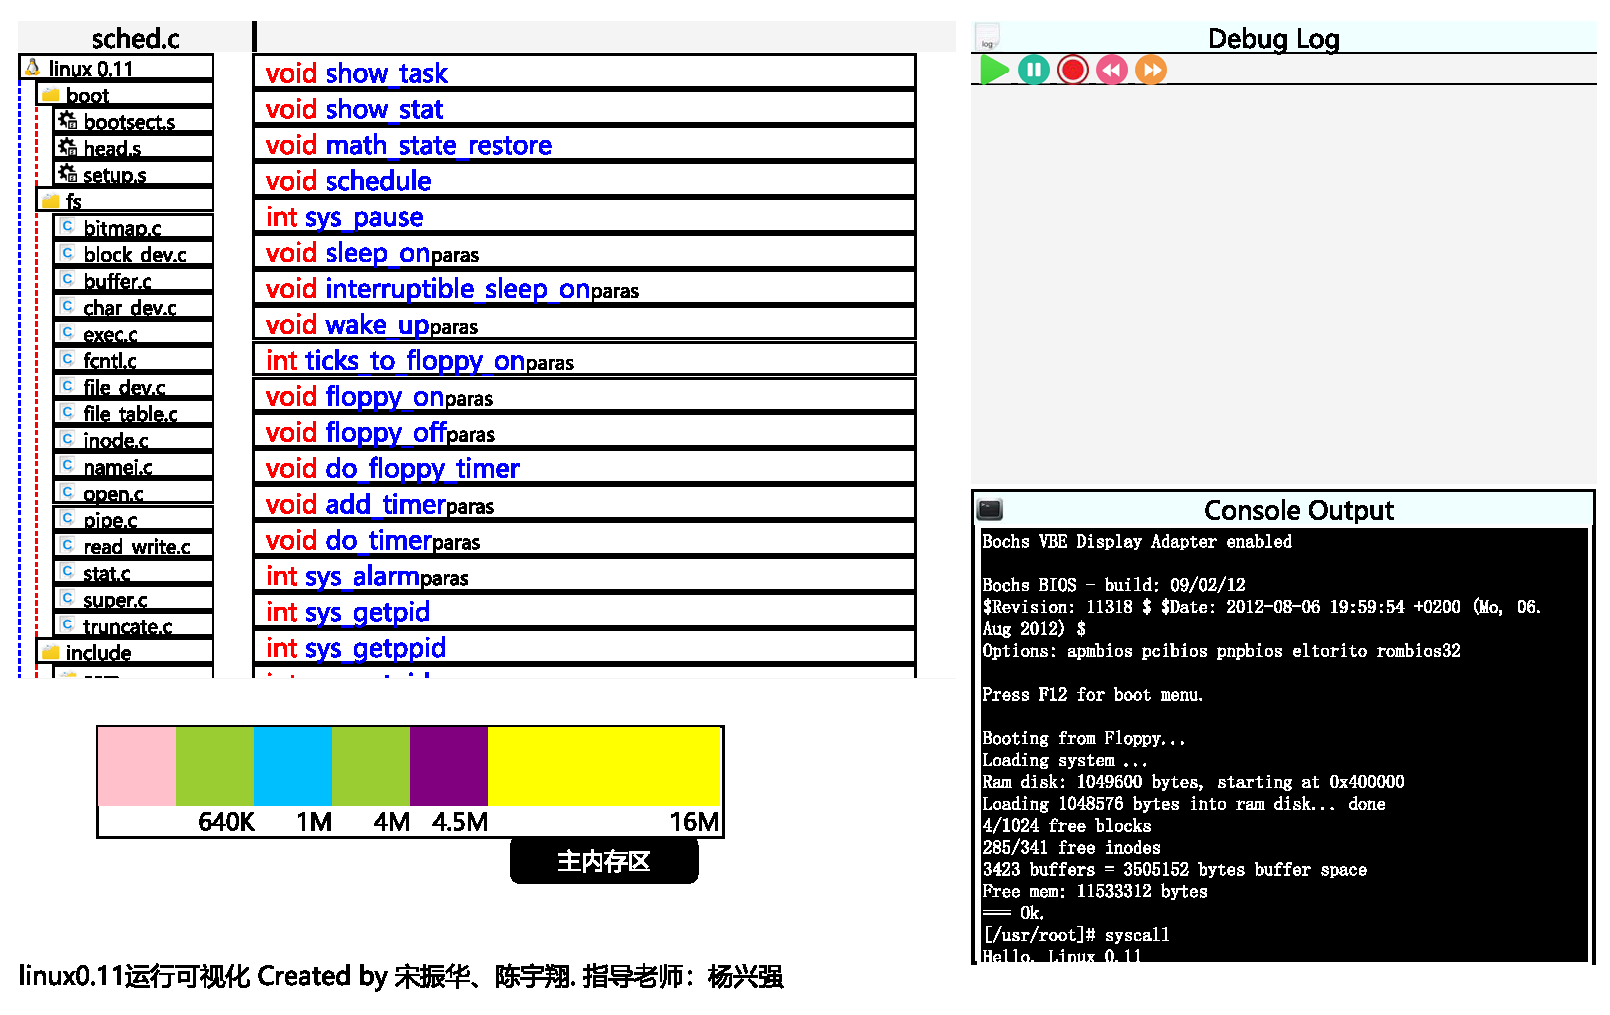
\includegraphics[width=\textwidth,natwidth=773 ,natheight=487]{img/index.html.pdf}
    \caption[]{主页, 包含对每个文件功能的介绍; 模拟内存及console}
    \label{fig:indexgraph}
\end{figure}

\begin{figure}[htbp]
    \centering
    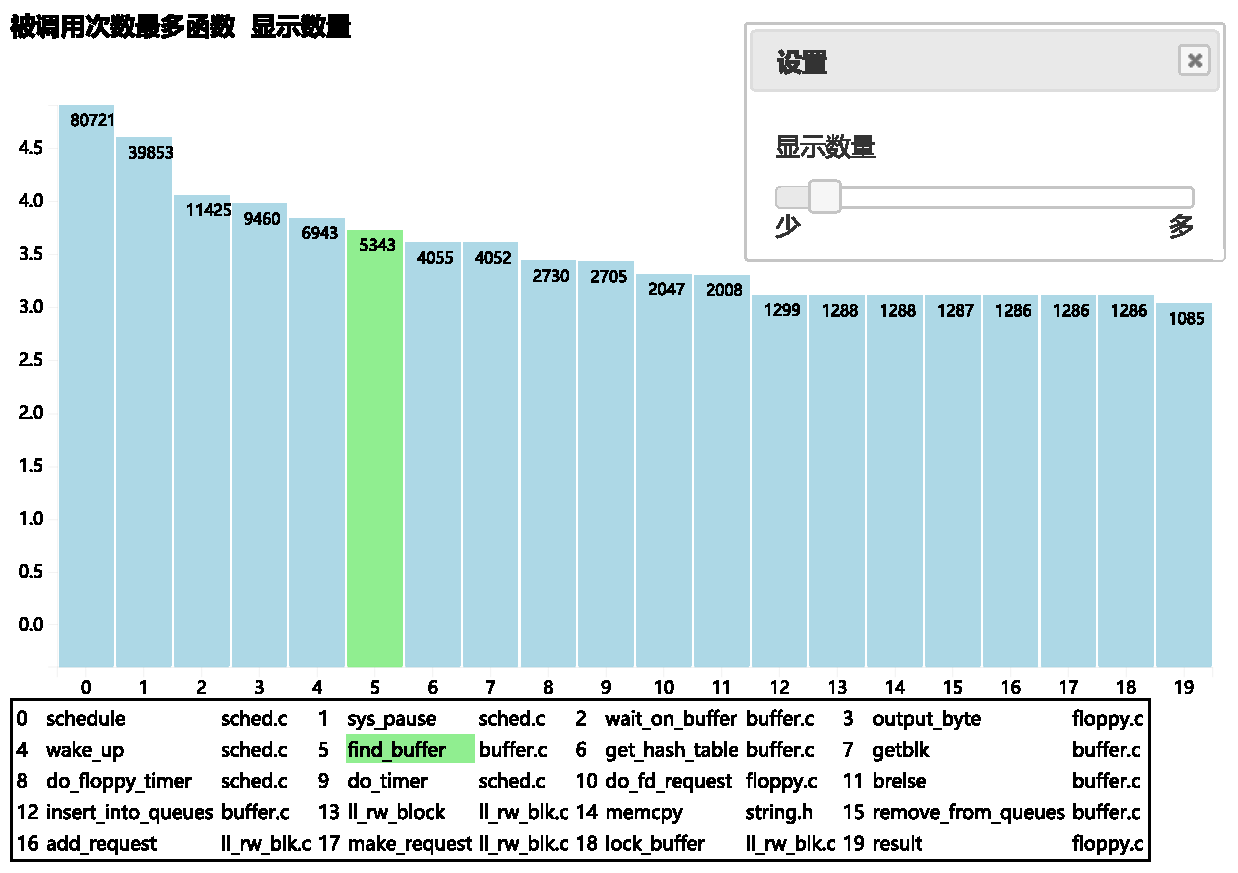
\includegraphics[width=\textwidth,natwidth=594 ,natheight=419]{img/calledMaxFunc.pdf}
    \caption[]{“引导界面调用次数最多”的函数 统计图. 表格与条形图可进行简单的交互. 纵坐标为log坐标轴}
    \label{fig:calledMaxFuncgraph}
\end{figure}

\begin{figure}[htbp]
    \centering
    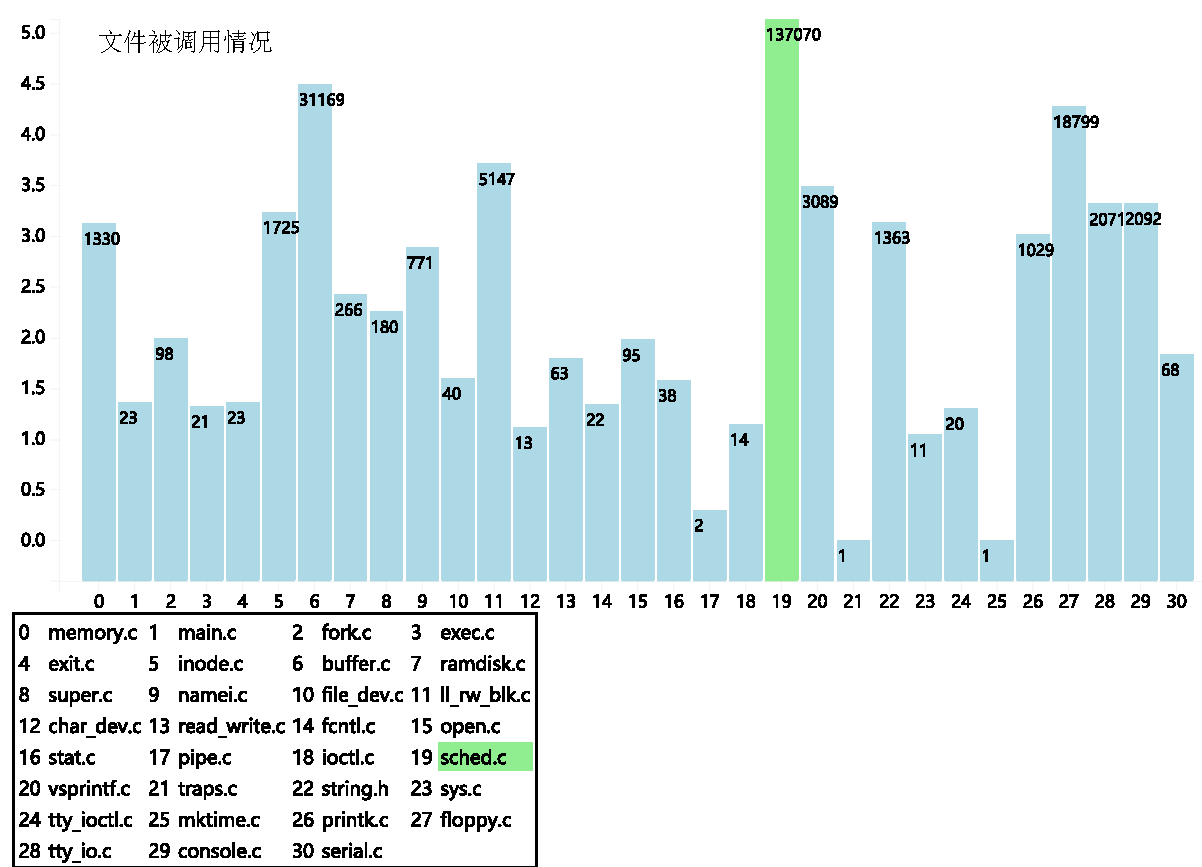
\includegraphics[width=\textwidth,natwidth=577 ,natheight=416]{img/calledFile.pdf}
    \caption[]{“引导界面调用次数最多”的文件 统计图}
    \label{fig:calledMaxFilegraph}
\end{figure}

\begin{figure}[htbp]
    \centering
    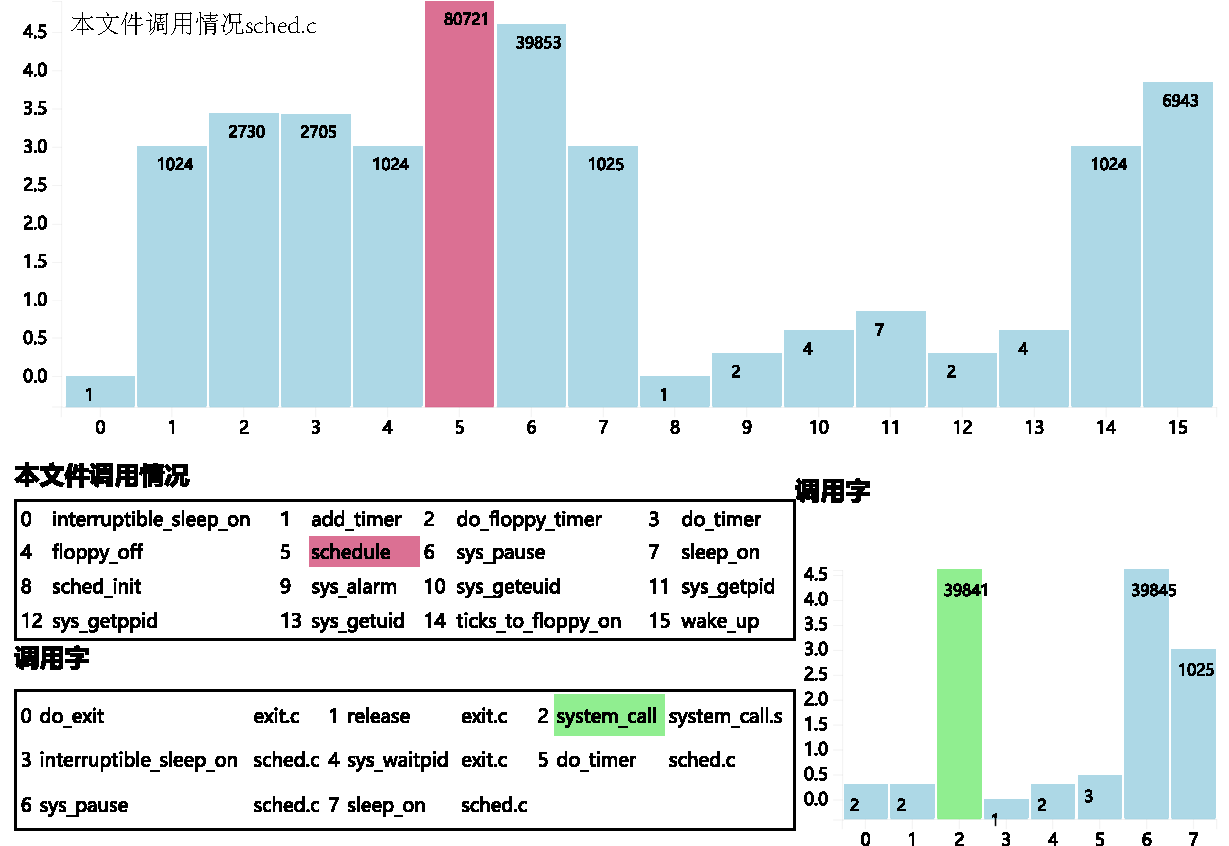
\includegraphics[width=\textwidth,natwidth=590 ,natheight=406]{img/eachFileCall.pdf}
    \caption[]{这是sched.c中函数统计调用图. 点击某函数, 可显示对应的调用字.}
    \label{fig:eachFileCallgraph}
\end{figure}

\begin{figure}[htbp]
    \centering
    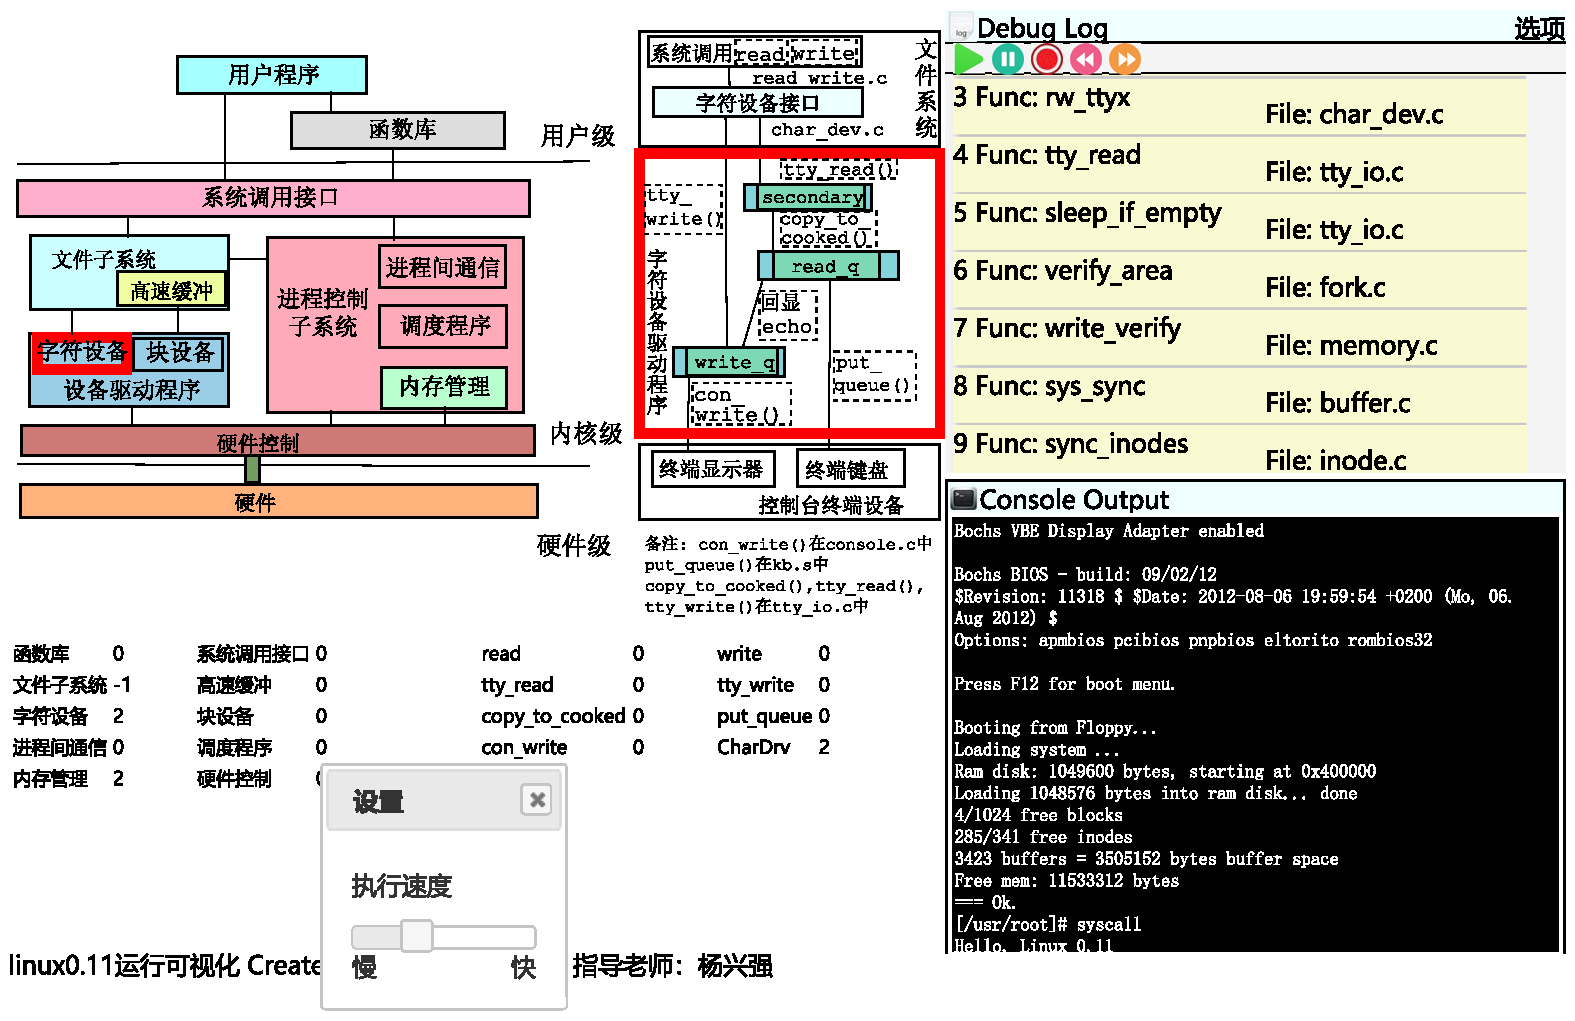
\includegraphics[width=\textwidth,natwidth=756 ,natheight=450]{img/chrdrv.pdf}
    \caption[]{字符设备动图}
    \label{fig:ChrDrvgraph}
\end{figure}

\chapter{系统运行过程实例}

不多说,直接上图

\begin{figure}
    \centering
    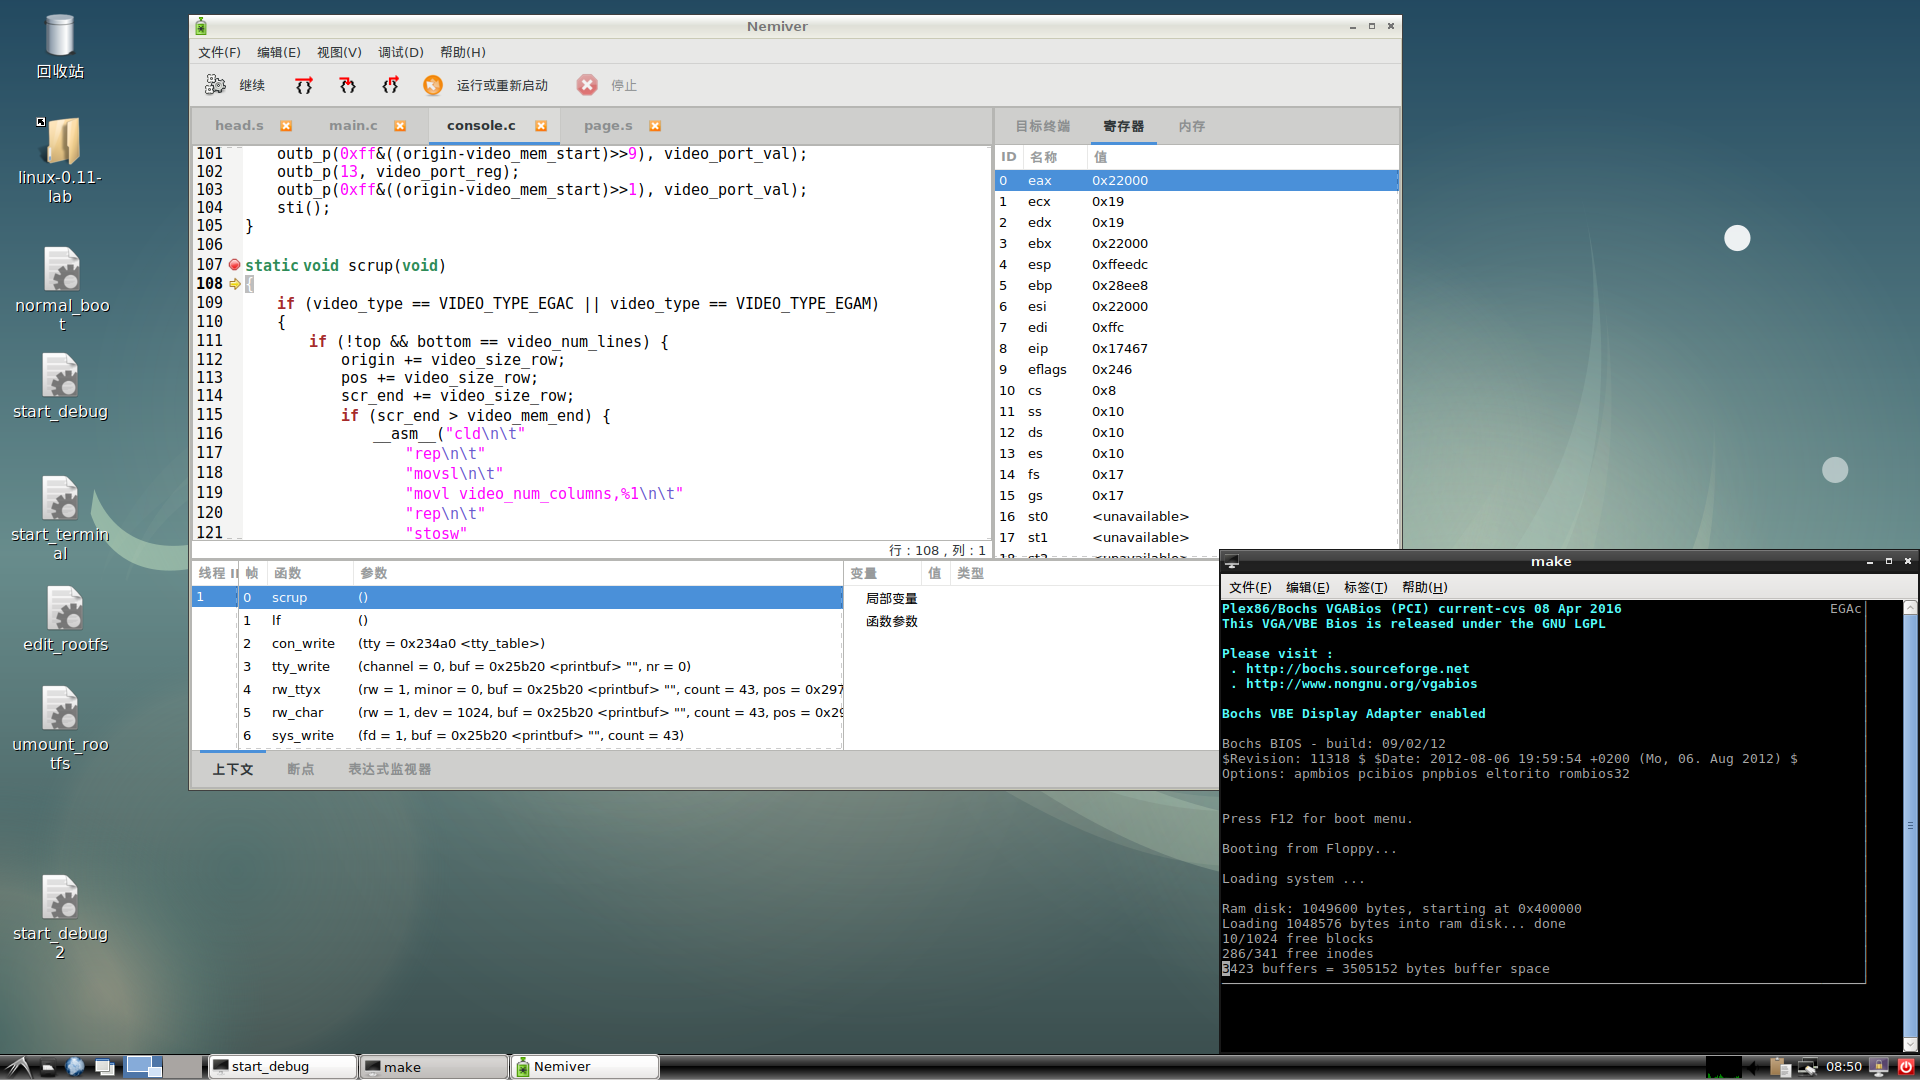
\includegraphics[width=1\linewidth]{img/1}
    \caption[图形化单步调试]{图形化单步调试}
    \label{fig:1}
\end{figure}
\begin{figure}
    \centering
    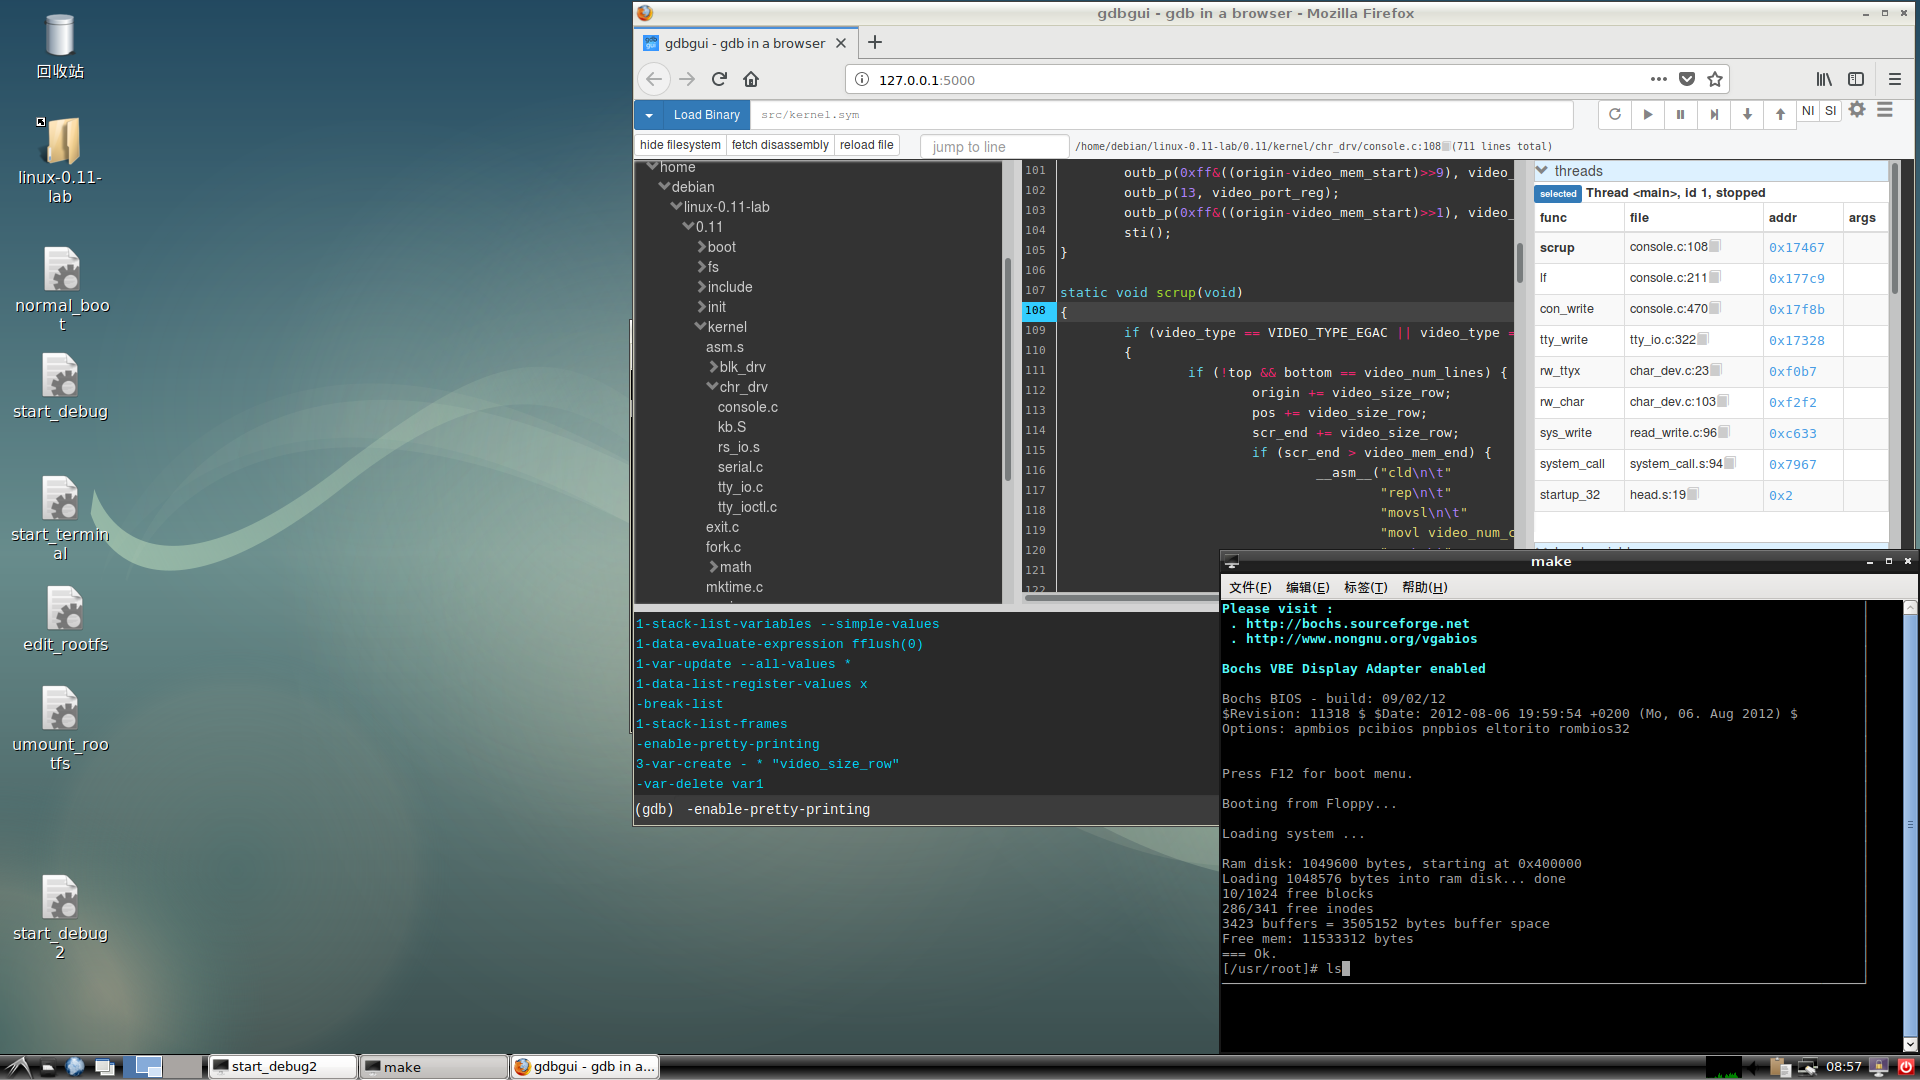
\includegraphics[width=1\linewidth]{img/2}
    \caption[图形化单步调试2]{图形化单步调试2}
    \label{fig:2}
\end{figure}
\begin{figure}
    \centering
    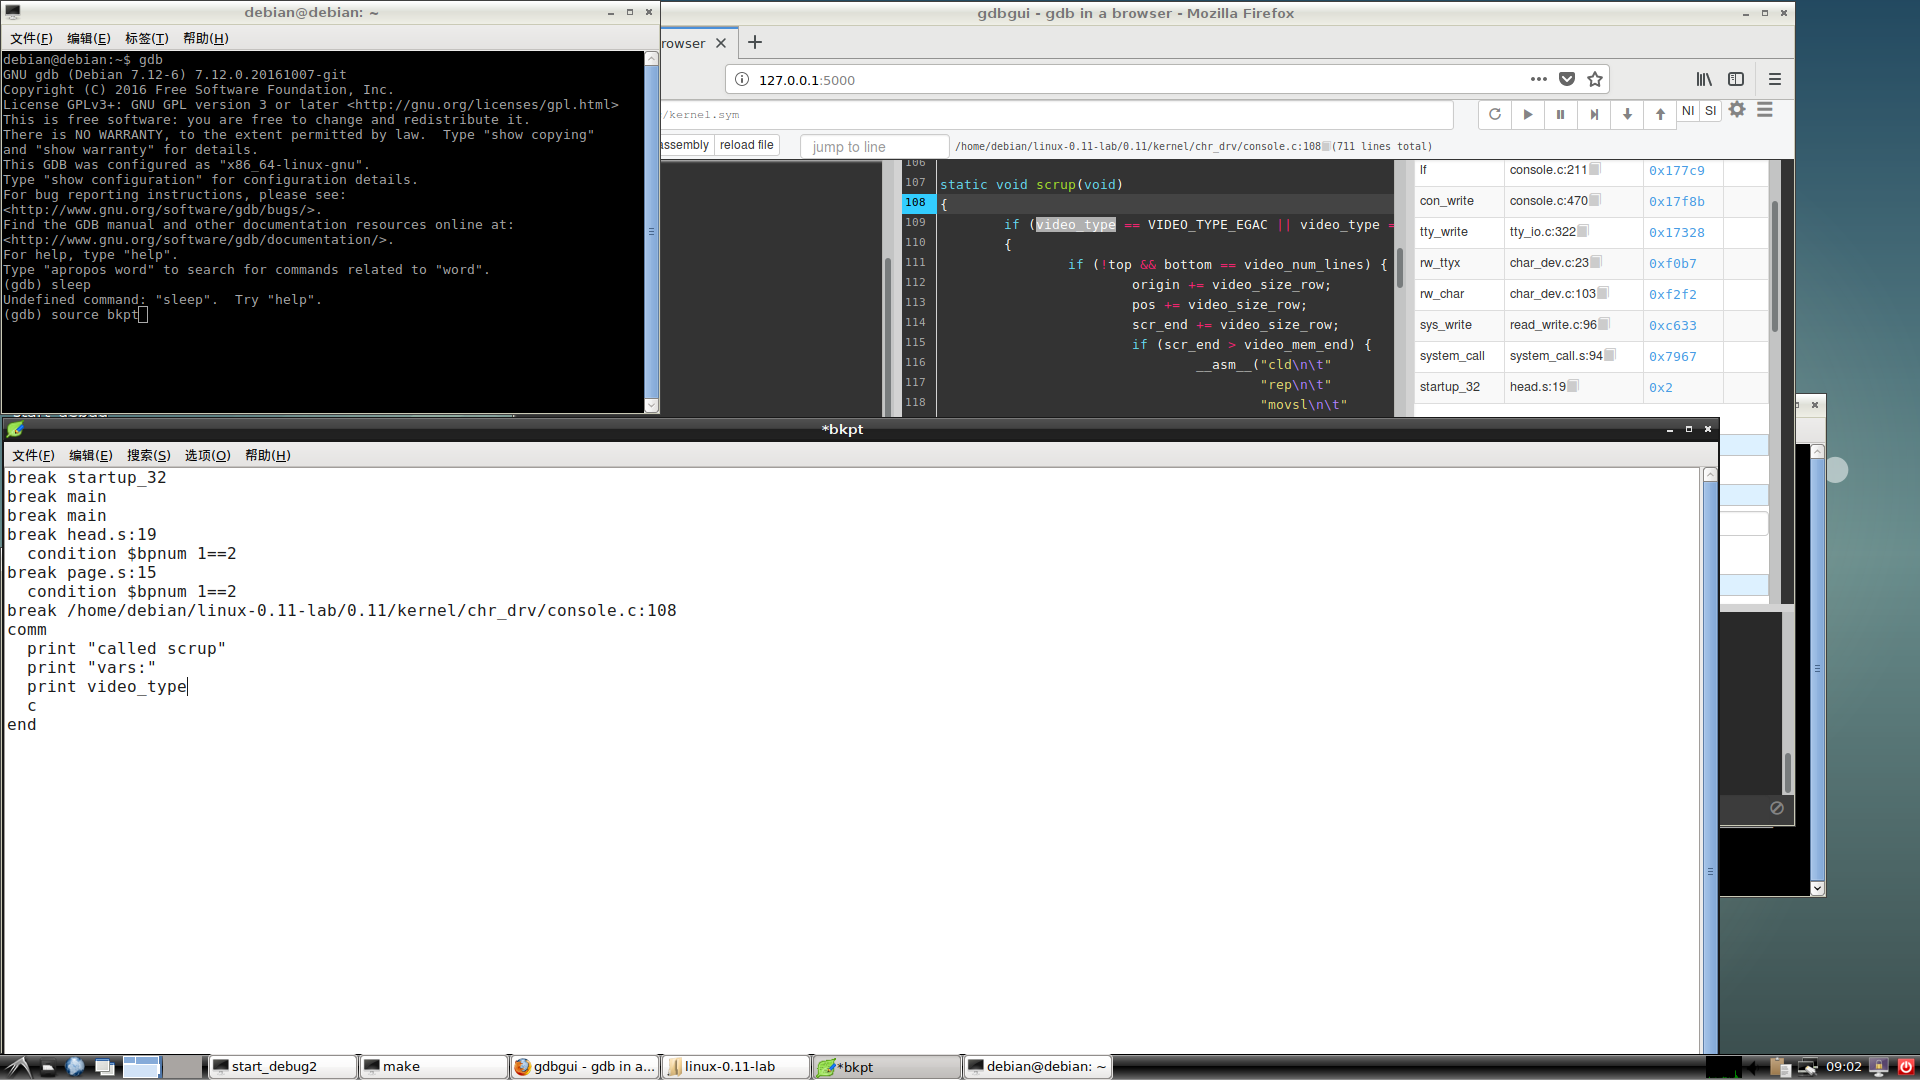
\includegraphics[width=1\linewidth]{img/3}
    \caption[手动使用GDB调试]{手动使用GDB调试}
    \label{fig:3}
\end{figure}
\begin{figure}
    \centering
    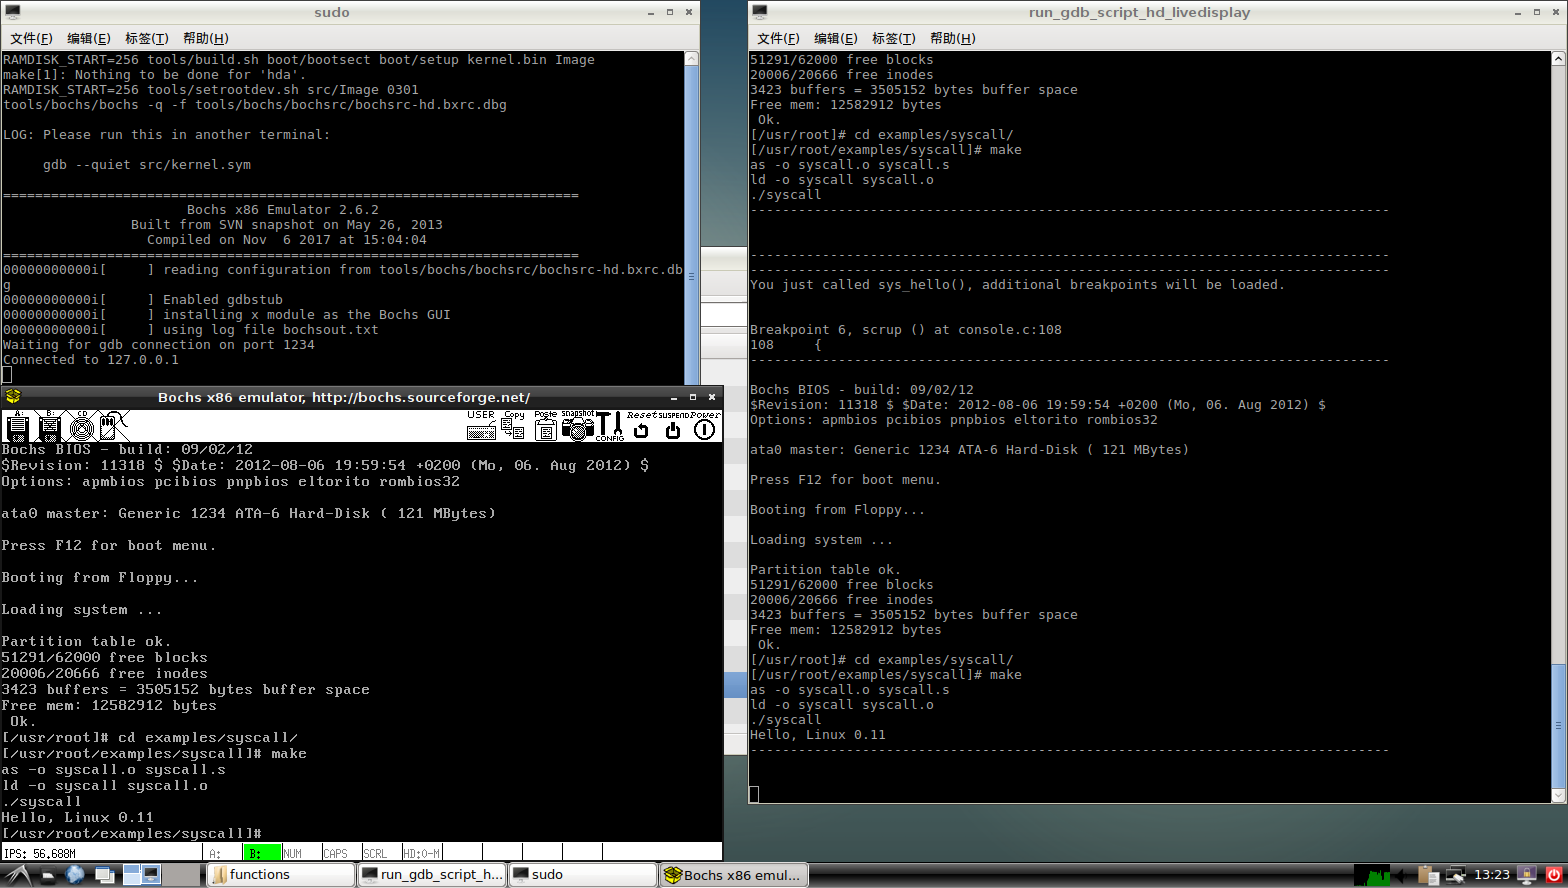
\includegraphics[width=1\linewidth]{img/4}
    \caption[启动脚本调试并调用sys\_call系统调用]{启动脚本调试并调用sys\_call系统调用}
    \label{fig:4}
\end{figure}


\end{document}          
